\chapter{Objetivos e características}

O gerenciamento dos recursos humanos do projeto inclui os processos para organizar, gerenciar e liderar a equipe do projeto, que são as pessoas com papéis e responsabilidades atribuídos para completar o projeto.

Os processos que fazem parte do gerenciamento dos recursos humanos, representados na Figura \ref{fig:proc:ger:rh}, podem ser resumidos em:

\begin{description}

	\item[Planejar o gerenciamento dos recursos humanos:] identificar e documentar os papéis, responsabilidades e habilidades requeridas, reportar relacionamentos e criar um plano de gerenciamento da equipe.
	
	\item[Mobilizar a equipe do projeto:] confirmar a disponibilidade dos recursos humanos e obter a equipe necessária para completar as atividades do projeto.
	
	\item[Desenvolver a equipe do projeto:] melhorar as competências, interação dos membros da equipe e ambiente geral da equipe para aprimorar o desempenho do projeto.
	
	\item[Gerenciar a equipe do projeto:] acompanhar o desempenho da equipe, fornecer feedback, resolver problemas e gerenciar mudanças para otimizar o desempenho do projeto.

\end{description}

\begin{figure}[!h]
	\centering
	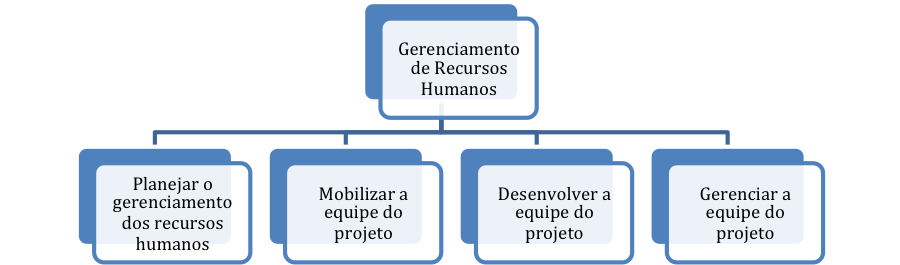
\includegraphics[scale=0.75]{Figuras/gerenciamento_rh.png}
	\caption{Processos do Gerenciamento dos recursos humanos}
	\label{fig:proc:ger:rh}
\end{figure}

\chapter{Planejar o gerenciamento dos recursos humanos}

Planejar o gerenciamento dos recursos humanos é o processo de identificar e documentar os papéis, responsabilidades e habilidades requeridas, reportar relacionamentos e criar um plano de gerenciamento da equipe.

O processo de planejar o gerenciamento dos recursos humanos está representado na Figura \ref{fig:rh:plan:efts} e será descrito a seguir.

\begin{figure}[!h]
	\centering
	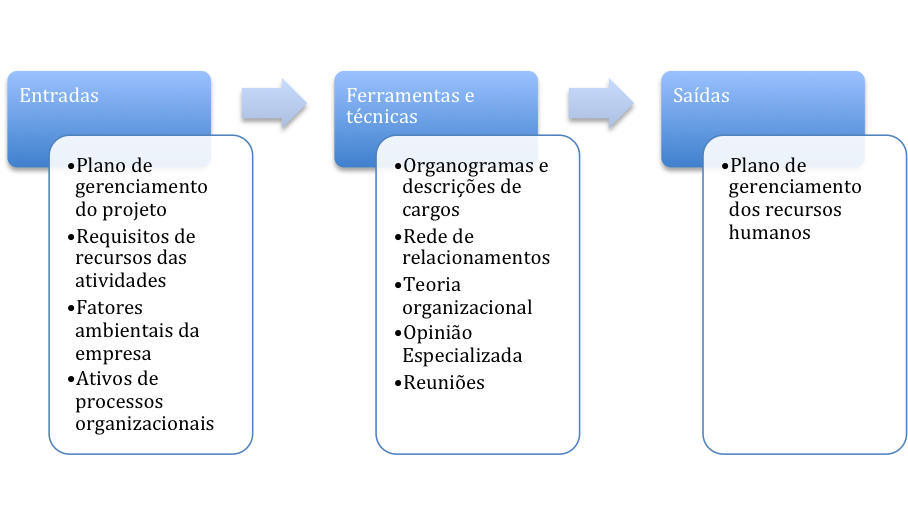
\includegraphics[scale=0.5]{Figuras/rh_efts_planejar.png}
	\caption{Planejar o gerenciamento dos recursos humanos: entradas, ferramentas, técnicas e saídas}
	\label{fig:rh:plan:efts}
\end{figure}

\section{Entradas}

\begin{description}
	
	\item[Plano de gerenciamento do projeto:] ciclo de vida e processos que serão aplicados em cada fase, como o trabalho será executado para alcançar os objetivos do projeto, plano de gerenciamento de mudanças que documenta como as mudanças serão monitoradas e controladas, plano de gerenciamento de configuração, como a integridade das linhas de base do projeto serão mantidas, necessidades e métodos de comunicação com as partes interessadas, etc.
	
	\item[Requisitos de recursos das atividades:] utilizado para determinar as necessidades de recursos humanos para o projeto.
	
	\item[Fatores ambientais da empresa:] cultura e estrutura organizacional, recursos humanos existentes, dispersão geográfica dos membros da equipe, políticas de administração de pessoal, condições de mercado, etc.
	
	\item[Ativos de processos organizacionais:] processos padronizados, políticas e descrições de papéis, modelos de organogramas e descrições de papéis, lições aprendidas sobre estruturas organizacionais que funcionaram em projetos anteriores, procedimentos de escalonamento para lidar com problemas dentro da equipe e dentro da organização, etc.
	

\end{description}

\section{Ferramentas e técnicas}

\begin{description}

	\item[Organogramas e descrições de cargos:] garantir que cada pacote de trabalho tenha um dono único e que todos os membros da equipe tenham uma compreensão clara de seus papéis e responsabilidades.
	
	\item[Rede de relacionamentos:] interações formais e informais com outras pessoas em uma organização, indústria ou ambiente profissional.
	
	\item[Teoria organizacional:] oferece informação a respeito da forma como as pessoas, equipes e unidades organizacionais se comportam.
	
	\item[Opinião Especializada:] listar requisitos preliminares para as habilidades necessárias, avaliar os papéis necessários para o projeto baseado em descrições padronizadas de papéis dentro da organização, determinar o nível de esforço preliminar e número de recursos necessários para alcançar os objetivos do projeto, determinar as subordinações necessárias baseado na cultura organzacional, oferecer orientações sobre o tempo necessário para formar a equipe, identificar riscos associados com a aquisição, retenção e desmobilização da equipe, identificar e recomendar programas para manter conformidade com contratos governamentais e sindicais, etc.
	
	\item[Reuniões:] podem ser necessárias durante o planejamento do gerenciamento dos recursos humanos.
	

\end{description}

\section{Saídas}

\begin{description}
	
	\item[Plano de gerenciamento dos recursos humanos:] plano contendo papéis e responsabilidades, organograma do projeto, plano de gerenciamento da equipe, etc.	
	
\end{description}

\chapter{Mobilizar a equipe do projeto}

Processo de confirmar a disponibilidade dos recursos humanos e obter a equipe necessária para completar as atividades do projeto.

O processo de mobilizar a equipe do projeto está representado na Figura \ref{fig:rh:mob:efts} e será descrito a seguir.

\begin{figure}[!h]
	\centering
	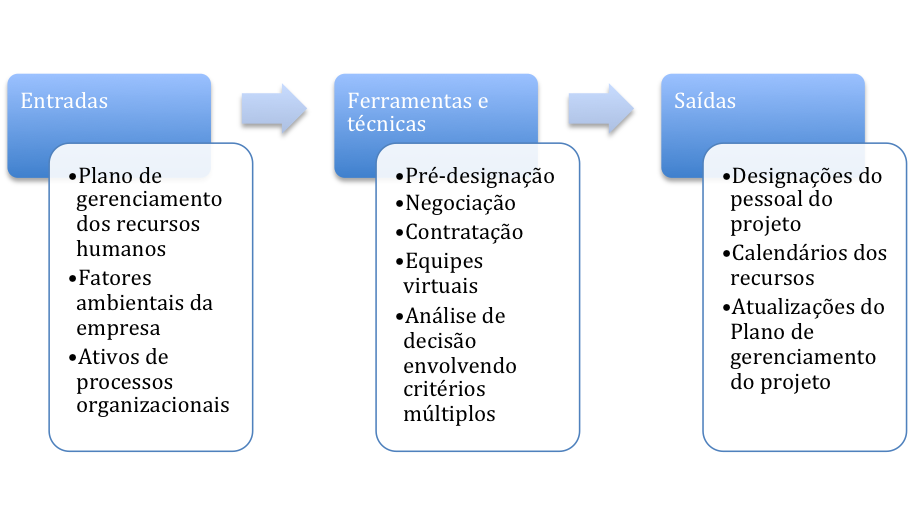
\includegraphics[scale=0.5]{Figuras/rh_efts_mobilizar.png}
	\caption{Mobilizar a equipe do projeto: entradas, ferramentas, técnicas e saídas}
	\label{fig:rh:mob:efts}
\end{figure}

\section{Entradas}

\begin{description}

	\item[Plano de gerenciamento dos recursos humanos:] oferece orientações sobre como os recursos humanos são identificados, compostos, gerenciados e eventualmente desmobilizados.
	
	\item[Fatores ambientais da empresa:] informações existentes sobre recursos humanos (disponibilidade, níveis de competência, experiência anterior, interesse em trabalhar no projeto e custos), políticas de administração de pessoal, estrutura organizacional, localização, etc.
	
	\item[Ativos de processos organizacionais:] políticas padronizadas da organização, processos, procedimentos, etc.
	
\end{description}

\section{Ferramentas e técnicas}

\begin{description}
	
	\item[Pré-designação:] ocorre quando os membros da equipe são selecionados com antecedência.
	
	\item[Negociação:] a negociação de atribuição de pessoal é necessária em diversos projetos.
	
	\item[Contratação:] quando a organização não consegue fornecer todo o pessoal necessário.
	
	\item[Equipes virtuais:] grupos de pessoas com objetivos compartilhados que cumprem seus papéis com pouco ou nenhum contato físico.
	
	\item[Análise de decisão envolvendo critérios múltiplos:] utilizados para dar notas ou pontuar potenciais membros da equipe e auxiliar na sua seleção.
	
\end{description}

\section{Saídas}

\begin{description}

	\item[Designações do pessoal do projeto:] a composição do projeto acontece quando as pessoas apropriadas forem designadas à equipe.
	
	\item[Calendários dos recursos:] documenta os períodos de tempo em que cada membro da equipe do projeto está disponível para o trabalho.
	
	\item[Atualizações do Plano de gerenciamento do projeto:] principalmente no plano de gerenciamento dos recursos humanos.
	
\end{description}

\chapter{Desenvolver a equipe do projeto}

Processo de melhorar as competências, interação dos membros da equipe e ambiente geral da equipe para aprimorar o desempenho do projeto.

O processo de desenvolver a equipe do projeto está representado na Figura \ref{fig:rh:desenv:efts} e será descrito a seguir.

\begin{figure}[!h]
	\centering
	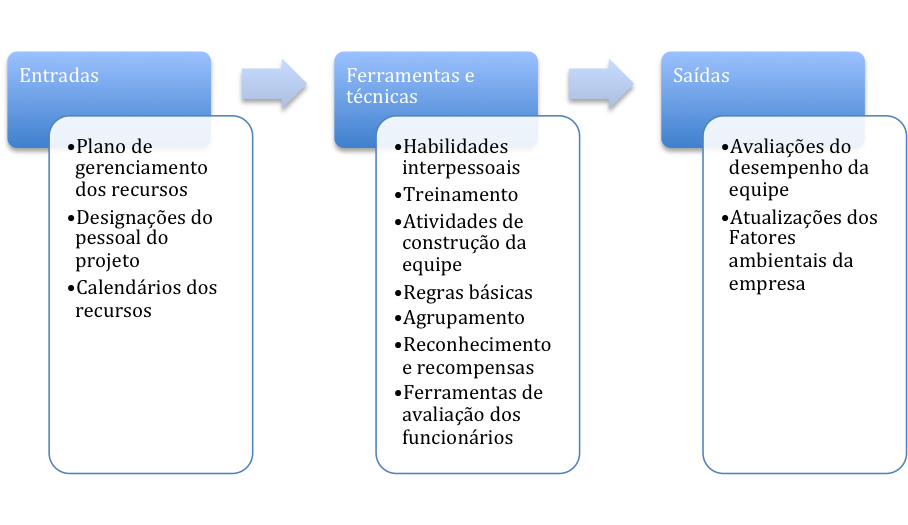
\includegraphics[scale=0.5]{Figuras/rh_efts_desenvolver.png}
	\caption{Desenvolver a equipe do projeto: entradas, ferramentas, técnicas e saídas}
	\label{fig:rh:desenv:efts}
\end{figure}

\section{Entradas}

\begin{description}

	\item[Plano de gerenciamento dos recursos:] define estratégias de treinamento e planos para desenvolvimento da equipe do projeto.
	
	\item[Designações do pessoal do projeto:] identifica as pessoas que estão na equipe.
	
	\item[Calendários dos recursos:] identifica períodos em que os membros da equipe podem participar de atividades de desenvolvimento.
	
	
\end{description}

\section{Ferramentas e técnicas}

\begin{description}
	
	\item[Habilidades interpessoais:] competências comportamentais tais como habilidades de comunicação, inteligência emocional, resolução de conflitos, negociação, influência, construção de equipes e facilitação de grupos.
	
	\item[Treinamento:] inclui todas as atividades para aumentar as competências dos membros da equipe.
	
	\item[Atividades de construção da equipe:] tem como objetivo auxiliar os membros individuais da equipe a trabalhar em conjunto eficientemente.
	
	\item[Regras básicas:] estabelece expectativas claras em relação ao comportamento aceitável da equipe do projeto.
	
	\item[Agrupamento:] envolve colocar muitos ou todos os membros mais ativos da equipe em um mesmo local físico para aumentar sua habilidade de trabalhar em equipe.
	
	\item[Reconhecimento e recompensas:] as pessoas são motivadas se elas se sentem valorizadas e essa valorização pode ser demonstrada através de recompensas (tangíveis ou intangíveis).
	
	\item[Ferramentas de avaliação dos funcionários:] oferecem uma percepção de áreas de força e fraqueza.
	
\end{description}

\section{Saídas}

\begin{description}
	
	\item[Avaliações do desempenho da equipe:] podem incluir indicadores tais como melhorias em habilidades que permitam executar tarefas mais efetivamente, melhorias em competências que auxiliam a equipe funcionar melhor como equipe, redução na taxa de rotatividade, aumento na coesão da equipe, etc.
	
	\item[Atualizações dos Fatores ambientais da empresa:] administração de pessoal, registros de treinamento de empregados, avaliação de habilidades, etc.
	
\end{description}

\chapter{Gerenciar a equipe do projeto}

É o processo de acompanhar o desempenho da equipe, fornecer feedback, resolver problemas e gerenciar mudanças para otimizar o desempenho do projeto.

O processo de gerenciar a equipe do projeto está representado na Figura \ref{fig:rh:ger:efts} e será descrito a seguir.

\begin{figure}[!h]
	\centering
	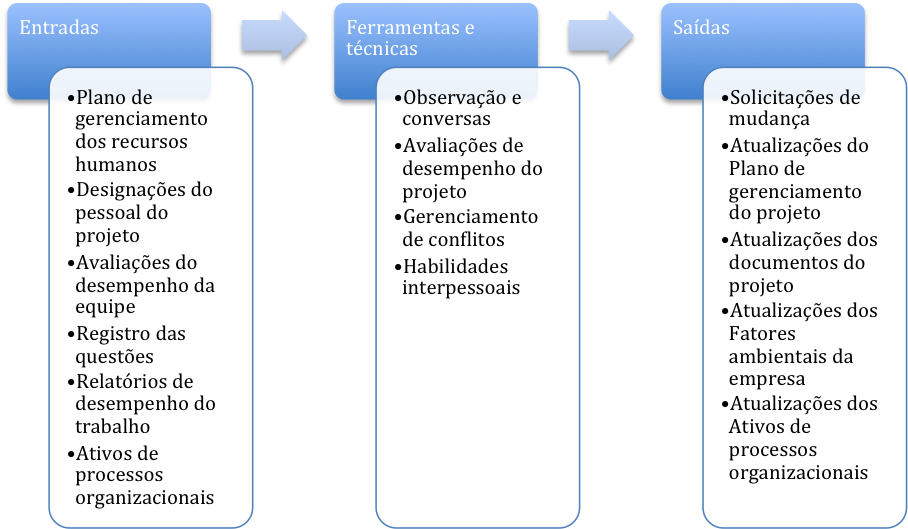
\includegraphics[scale=0.5]{Figuras/rh_efts_gerenciar.png}
	\caption{Gerenciar a equipe do projeto: entradas, ferramentas, técnicas e saídas}
	\label{fig:rh:ger:efts}
\end{figure}

\section{Entradas}

\begin{description}

	\item[Plano de gerenciamento dos recursos humanos:] inclui os papéis e responsabilidades, organização do projeto, plano de gerenciamento do pessoal, etc.
	
	\item[Designações do pessoal do projeto:] inclui a lista dos membros da equipe.
	
	\item[Avaliações do desempenho da equipe:] através da avaliação contínua do desempenho da equipe, ações podem ser tomadas para resolver problemas, modificar a comunicação, resolver conflitos e melhorar a interação da equipe.
	
	\item[Registro das questões:] usada para documentar e monitorar quem é responsável pela resolução de problemas específicos em uma data limite.
	
	\item[Relatórios de desempenho do trabalho:] auxilia na determinação de futuras necessidades de pessoal, reconhecimentos e recompensas e atualizações no plano de gerenciamento de pessoal.
	
	\item[Ativos de processos organizacionais:] certificados de apreciação, jornais internos, sites, estruturas de bônus, etc.
	
\end{description}

\section{Ferramentas e técnicas}

\begin{description}

	\item[Observação e conversas:] são usadas para manter contato com o trabalho e atitudes dos membros da equipe.
	
	\item[Avaliações de desempenho do projeto:] tem como objetivo clarificar os papéis e responsabilidades, fornecer feedback construtivo, descobrir problemas desconhecidos ou não resolvidos, desenvolver planos de treinamento e estabelecer objetivos específicos para períodos futuros.
	
	\item[Gerenciamento de conflitos:] resulta em uma maior produtividade e relacionamentos de trabalho positivos.
	
	\item[Habilidades interpessoais:] incluem principalmente liderança, influência e tomada de decisão efetiva.
		
\end{description}

\section{Saídas}

\begin{description}

	\item[Solicitações de mudança:] mudanças na equipe podem impactar no projeto e alterar o cronograma ou orçamento.
	
	\item[Atualizações do Plano de gerenciamento do projeto:] principalmente no plano de gerenciamento de recursos humanos.
	
	\item[Atualizações dos documentos do projeto:] registro de questões, descrição de papéis, designação de pessoal, etc.
	
	\item[Atualizações dos Fatores ambientais da empresa:] entrada para avaliação de desempenho organizacional, competências de pessoal, etc.
	
	\item[Atualizações dos Ativos de processos organizacionais:] informações históricas, lições aprendidas, modelos, processos padronizados, etc.
	
	
\end{description}